\begin{frame}
    \frametitle{What is dolfin-adjoint?}

    Dolfin-adjoint is an extension of FEniCS for: solving adjoint and
    tangent linear equations; generalised stability analysis;
    PDE-constrained optimisation.

    \begin{block}{Main features}
        \begin{itemize}
            \item Automated derivation of first and second order adjoint and tangent linear models.
            \item Discretely consistent derivatives.
            \item Parallel support and near theoretically optimal performance.
            \item Interface to optimisation algorithms for PDE-constrained optimisation.
            \item Documentation and examples on \url{www.dolfin-adjoint.org}.
        \end{itemize}
    \end{block}

\end{frame}

\begin{frame}
    \frametitle{What has dolfin-adjoint been used for?}
    \framesubtitle{Layout optimisation of tidal turbines}
    \begin{figure}
    \begin{center}
        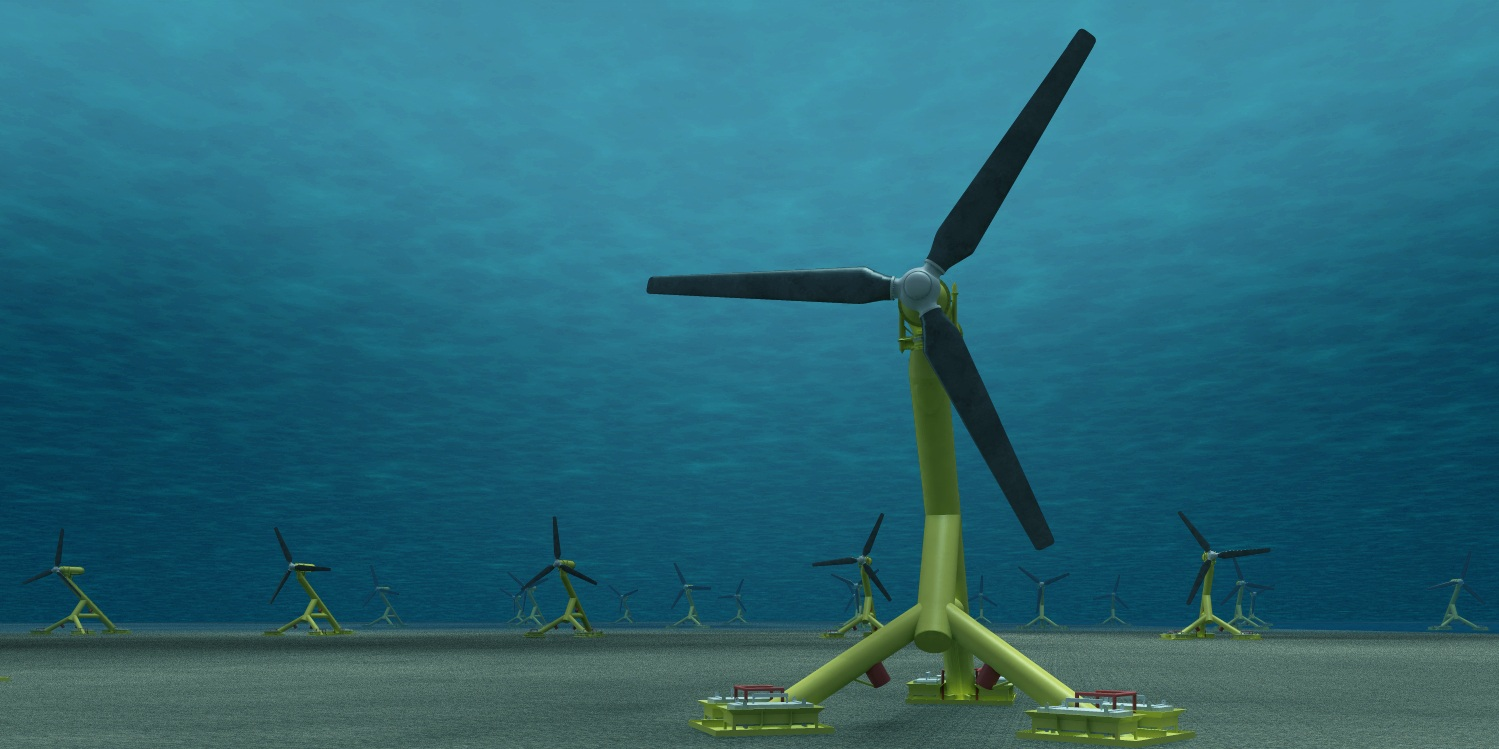
\includegraphics[width=0.45\textwidth]{jpg/tidal_farm}
        \hspace{1cm}
        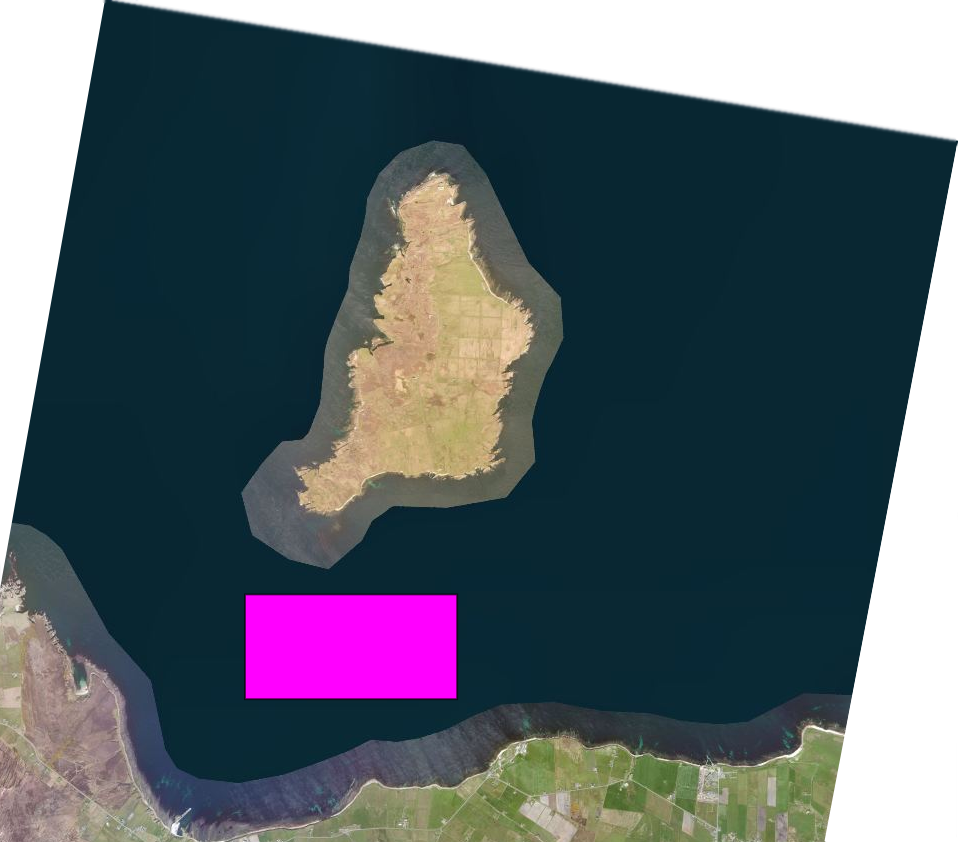
\includegraphics[width=0.25\textwidth]{png/satellite}
    \end{center}
    \end{figure}
        \begin{itemize}
            \item Up to 400 tidal turbines in one farm.
            \item What are the optimal locations to maximise power production?
        \end{itemize}
\end{frame}

\begin{frame}
    \frametitle{What has dolfin-adjoint been used for?}
    \framesubtitle{Layout optimisation of tidal turbines}
    \begin{center}
        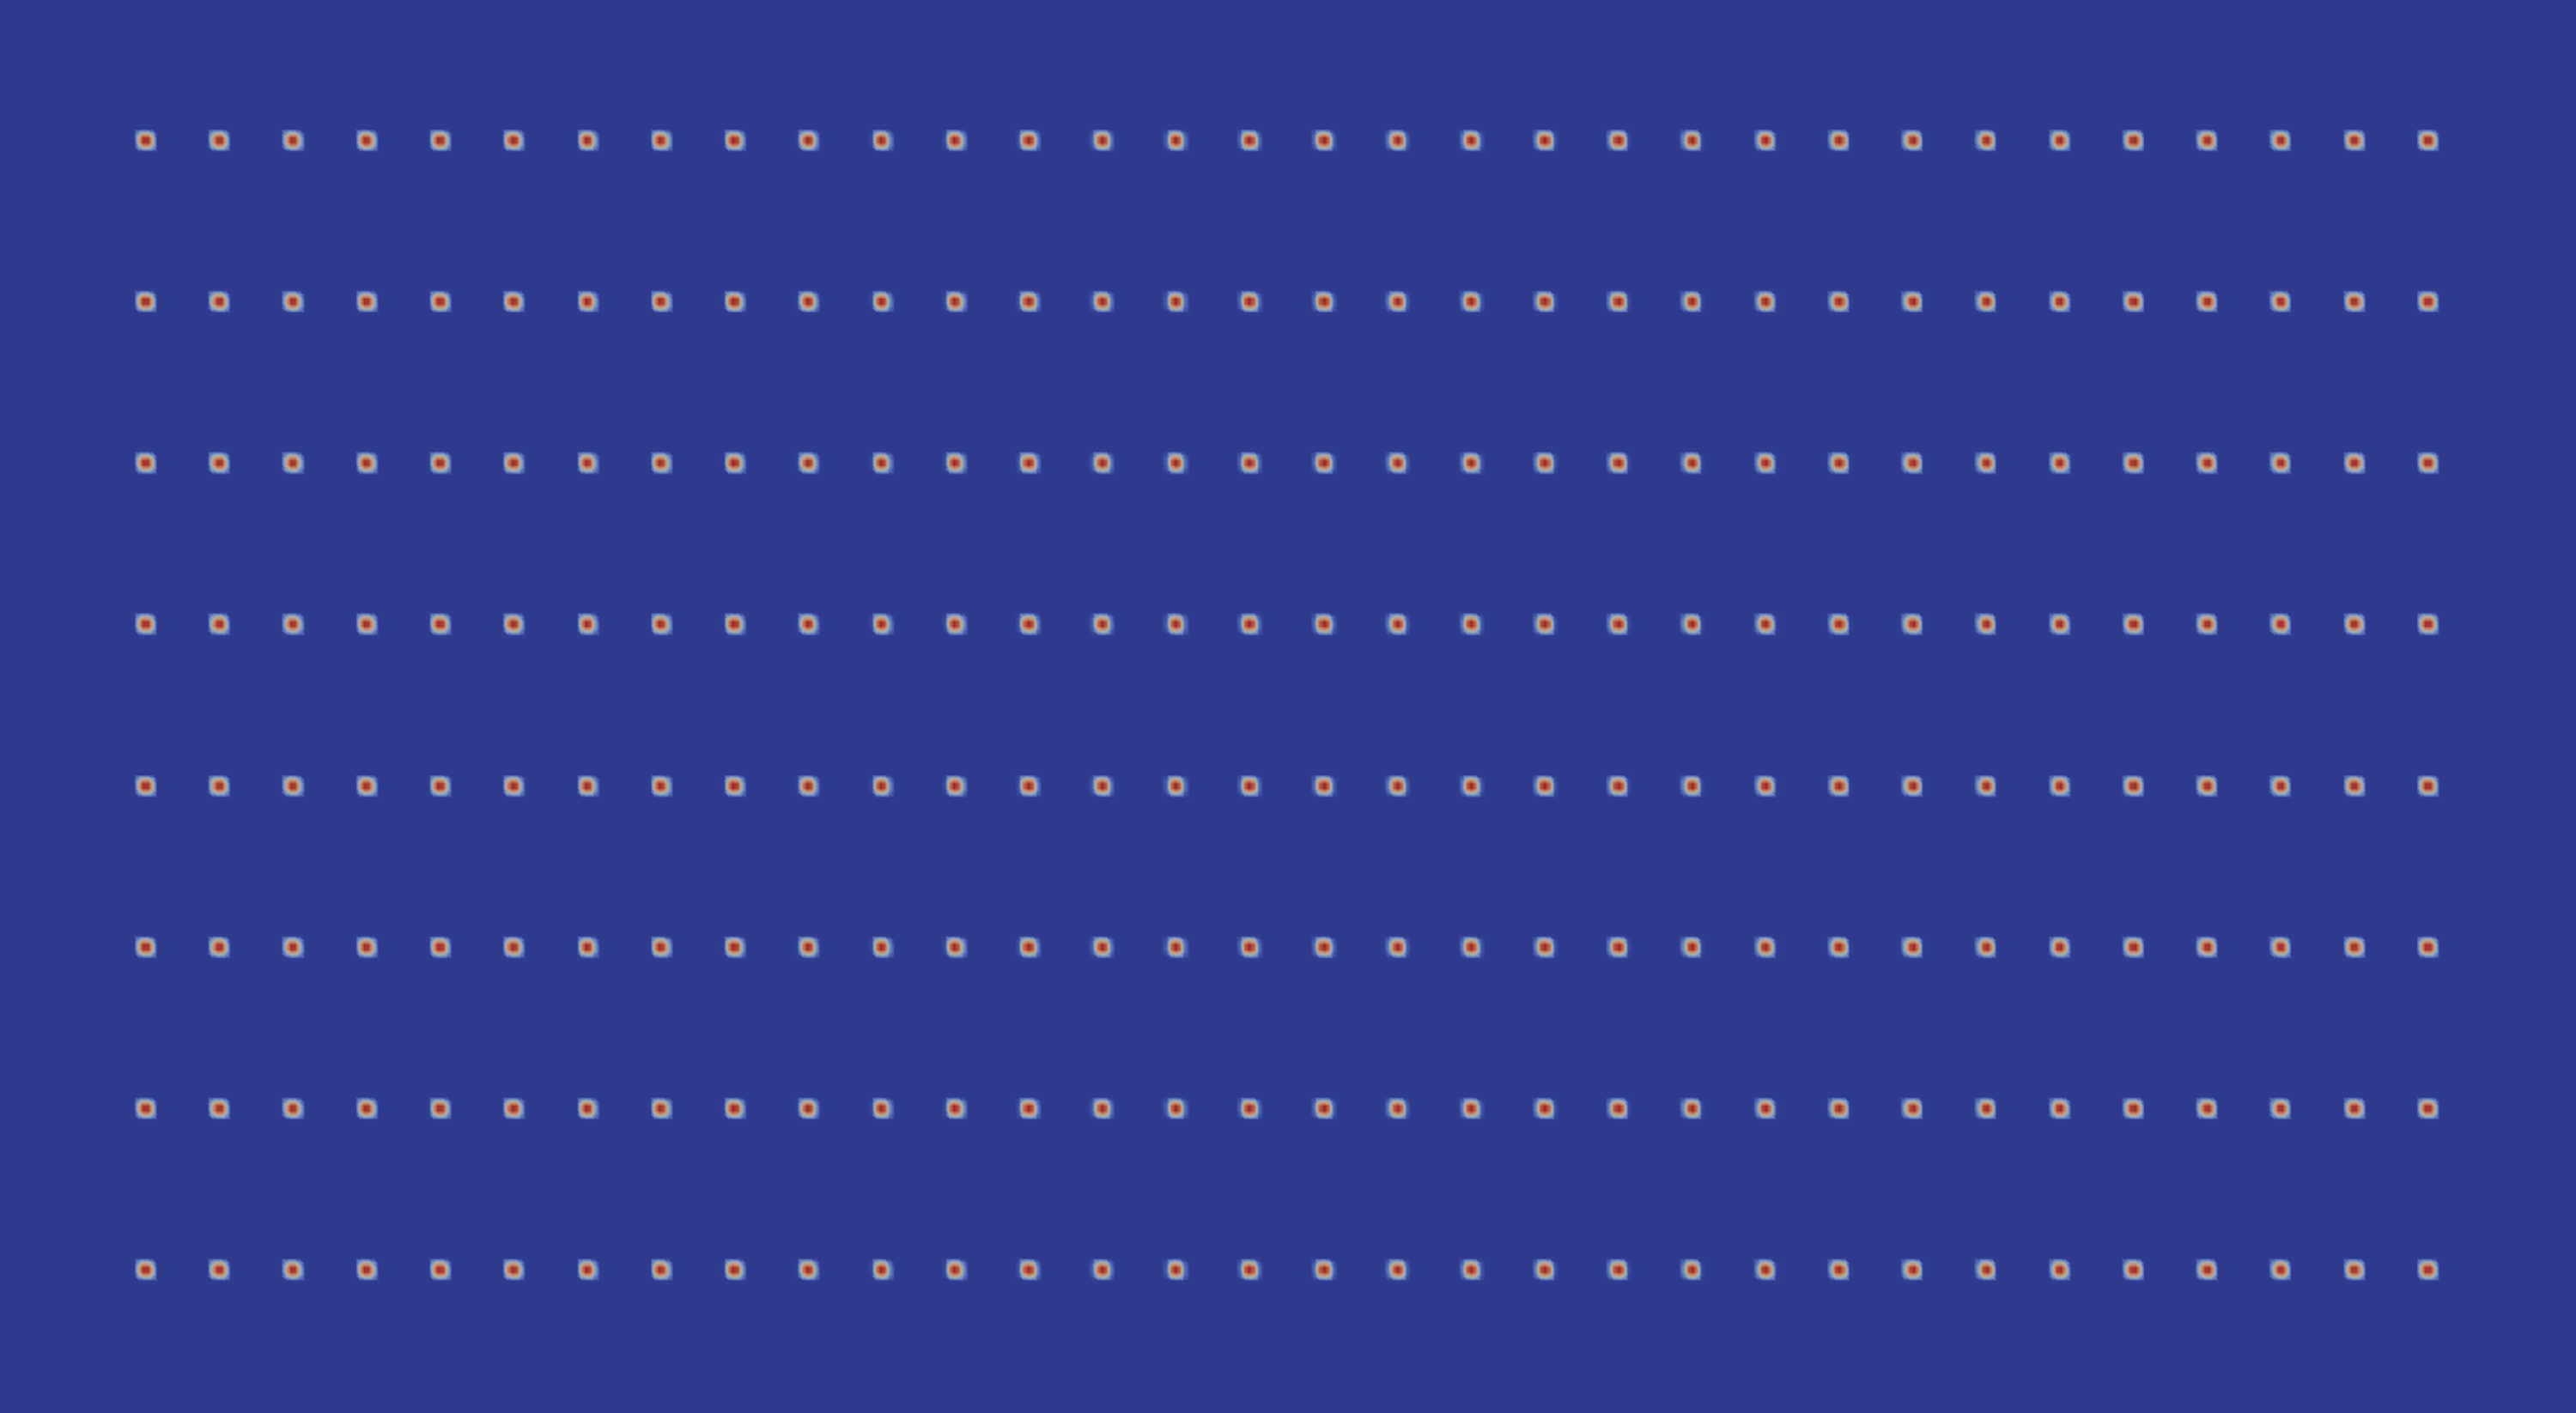
\includegraphics[width=0.35\textwidth]{png/turbine0}
        \hspace{1cm}
        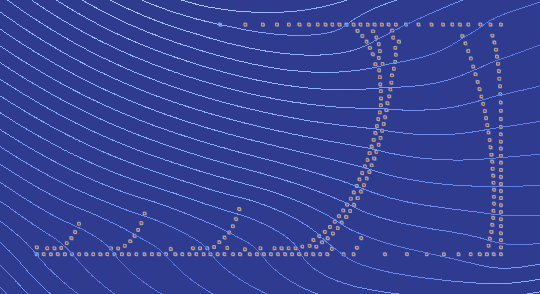
\includegraphics[width=0.35\textwidth]{png/streamlines_zoomed} \\
        \vspace{1cm}
        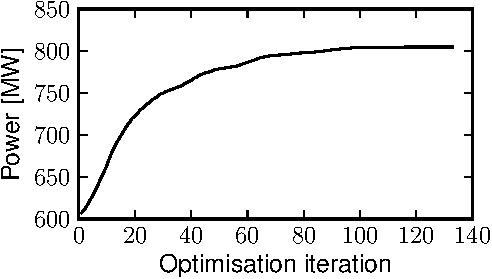
\includegraphics[width=0.45\textwidth]{pdf/OpenTidalFarm_iterplot}
    \end{center}
\end{frame}

\begin{frame}[fragile]
    \frametitle{What has dolfin-adjoint been used for?}
    \framesubtitle{Layout optimisation of tidal turbines}
\begin{python}
from dolfin import *
from dolfin_adjoint import *

# FEniCS model
# ...

J = Functional(turbines*inner(u, u)**(3/2)*dx*dt)
m = Control(turbine_positions)
R = ReducedFunctional(J, m)
maximize(R)
\end{python}

\end{frame}


\frame
{
  \frametitle{What has dolfin-adjoint been used for?}
  \framesubtitle{Reconstruction of a tsunami wave}
        \begin{center}
        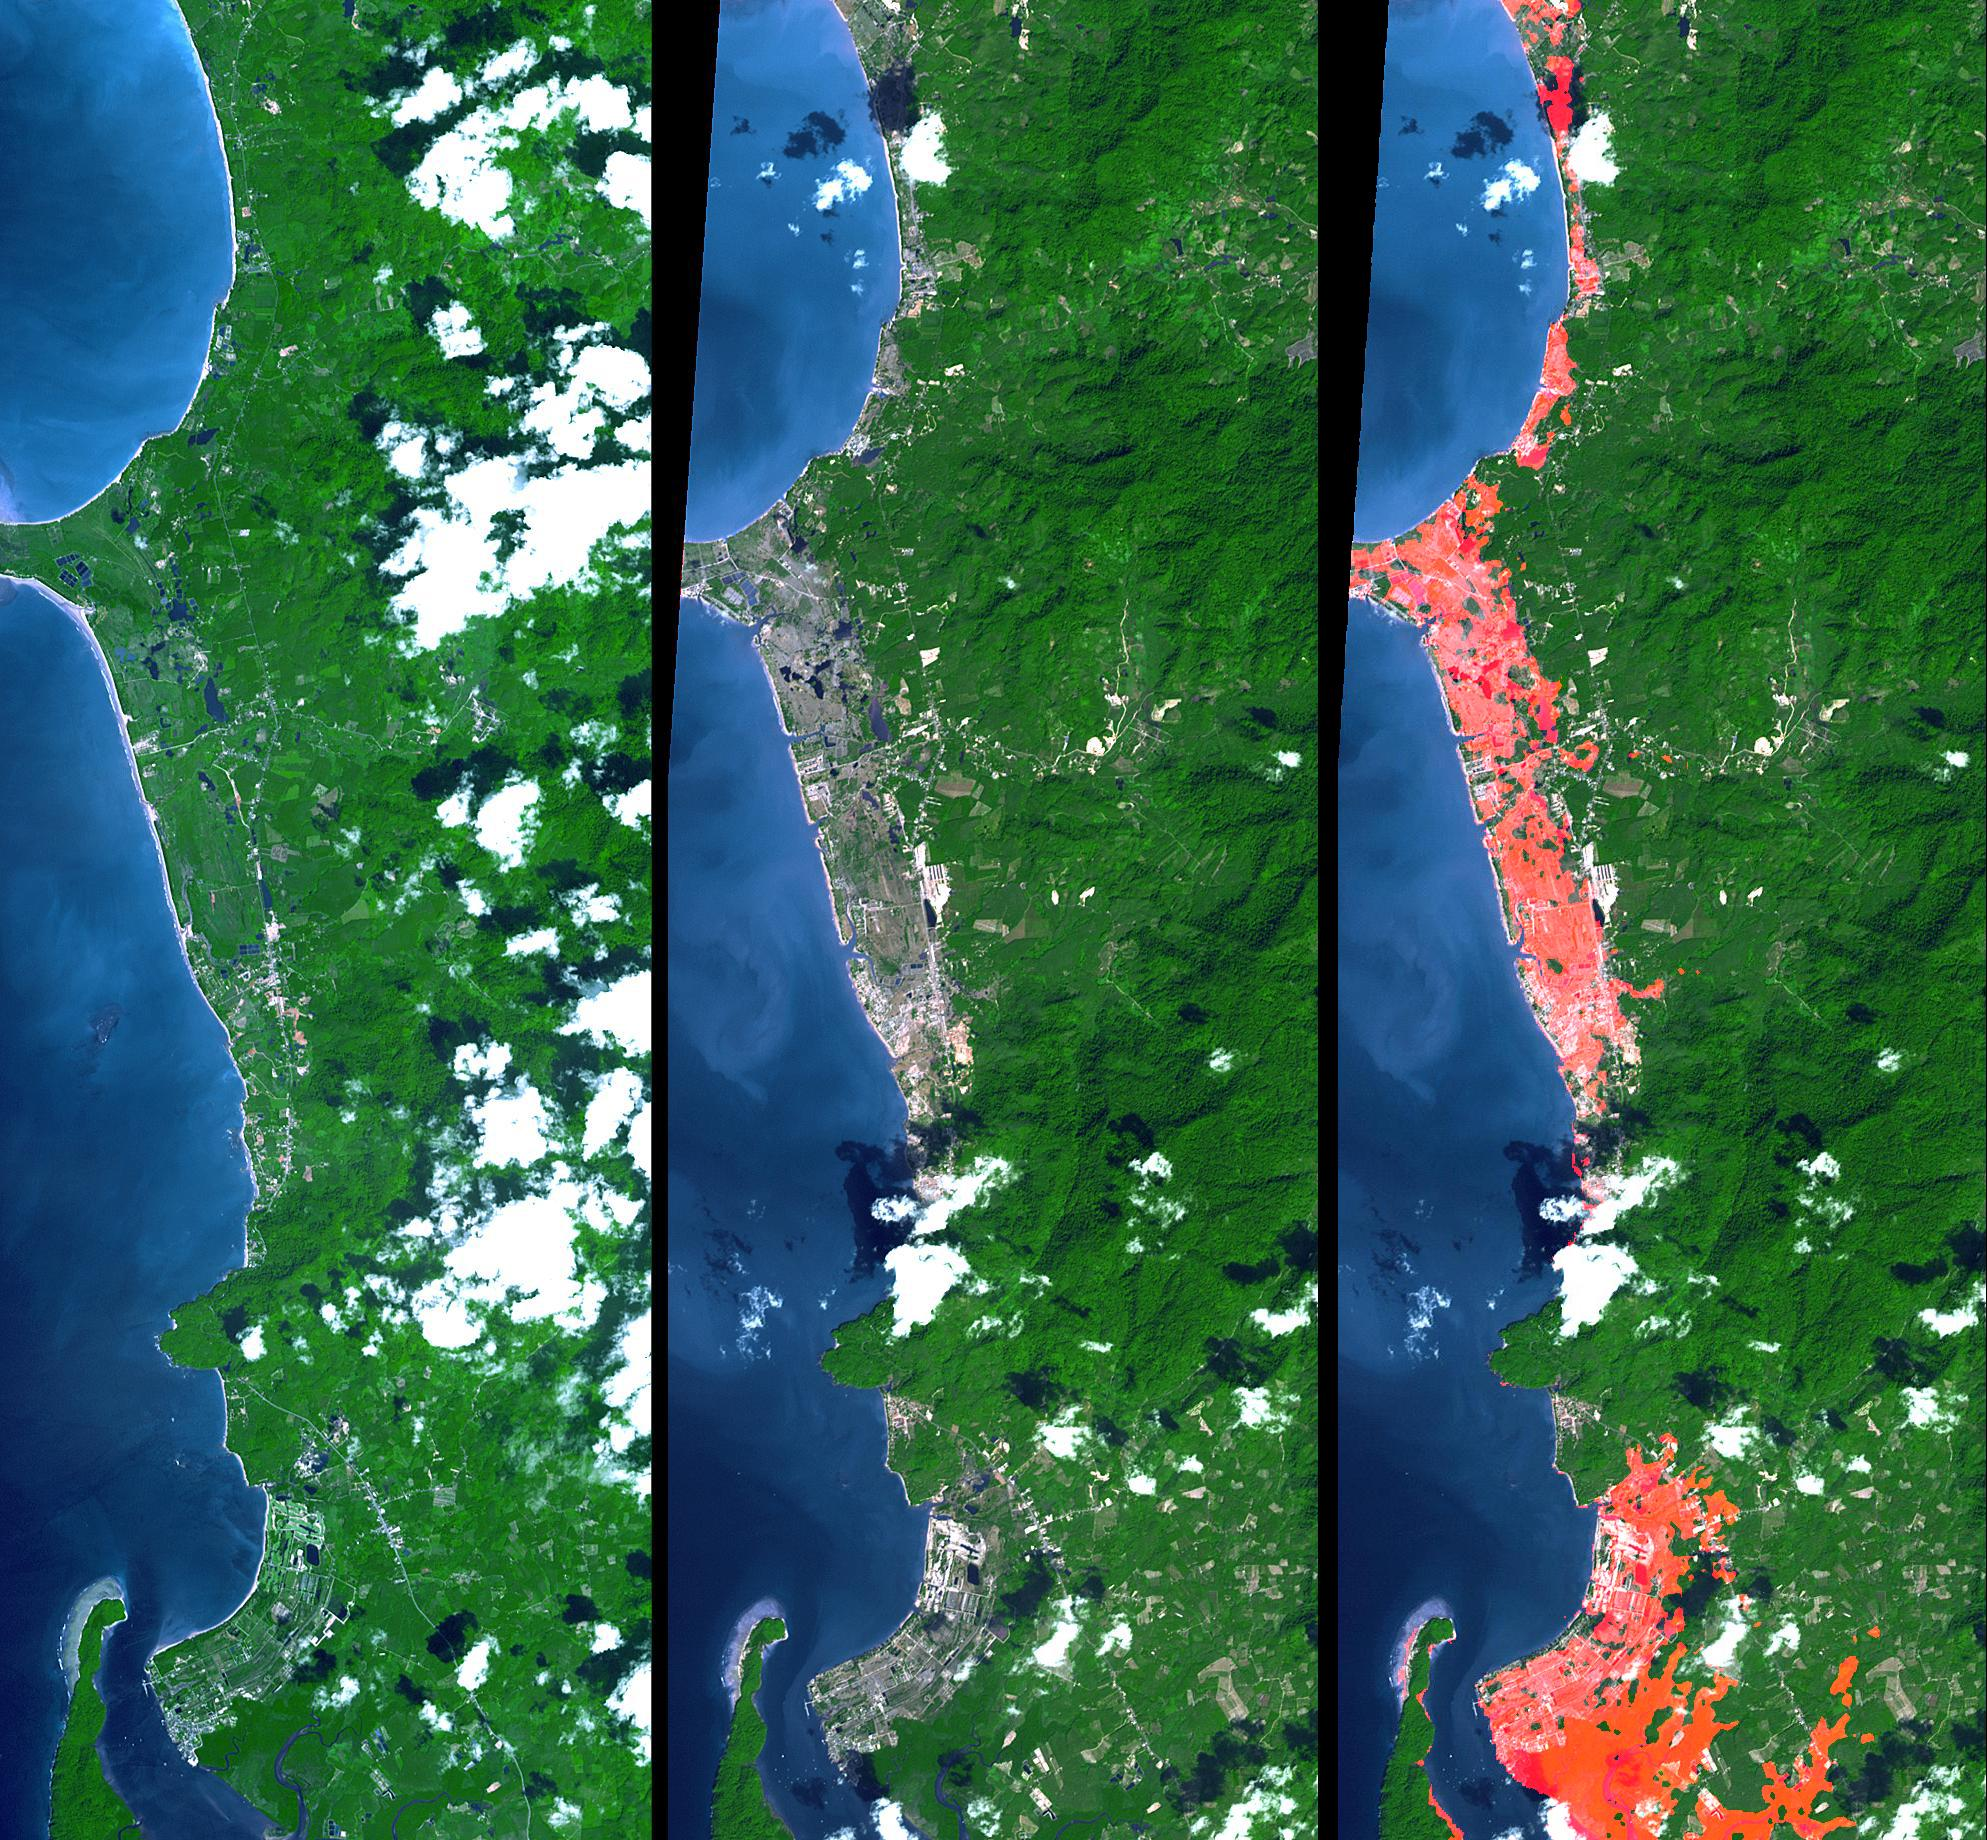
\includegraphics[width=0.55\textwidth]{jpg/PIA06671}\footnote{Image: ASTER/NASA PIA06671} \\
        Is it possible to reconstruct a tsunami wave from images like this?
        \end{center}
}

\frame
{
  \frametitle{What has dolfin-adjoint been used for?}
  \framesubtitle{Reconstruction of a tsunami wave}
        \begin{center}
        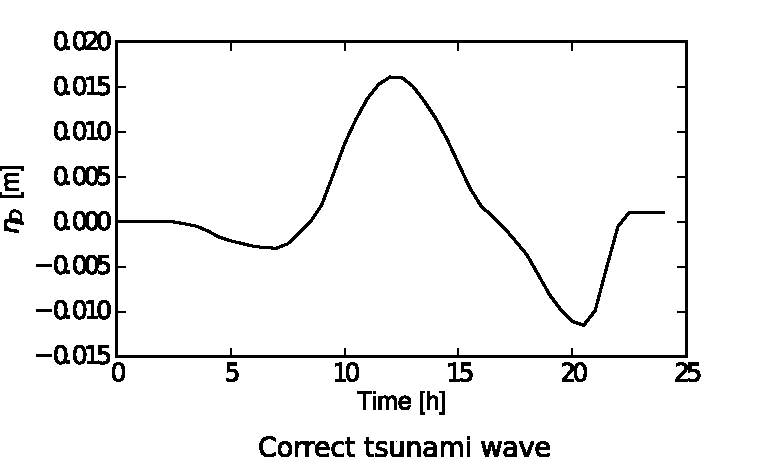
\includegraphics[width=0.45\textwidth]{pdf/controls_optimal}
        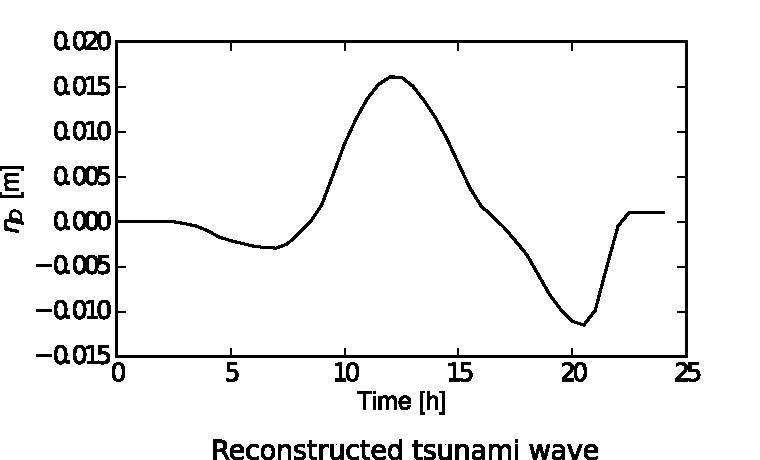
\includegraphics[width=0.45\textwidth]{pdf/controls_47} \\
        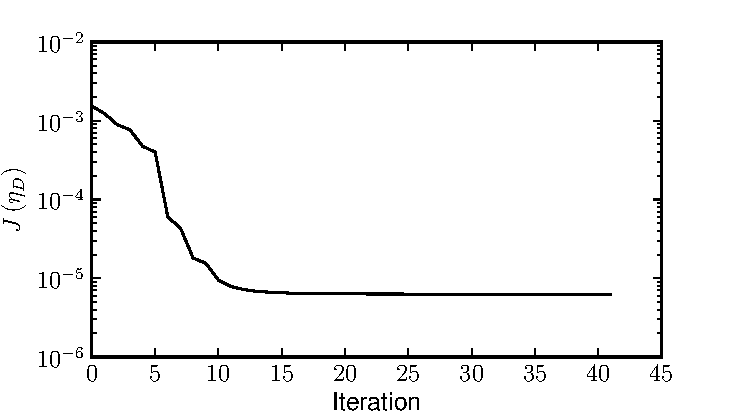
\includegraphics[width=0.45\textwidth]{pdf/wetdry_iter_plot} \\
        \end{center}
}

\begin{frame}[fragile]
  \frametitle{Reconstruction of a tsunami wave}
  \begin{python}
from fenics import *
from dolfin_adjoint import *

# FEniCS model
# ...

J = Functional(observation_error**2*dx*dt)
m = Control(input_wave)
R = ReducedFunctional(J, m)
minimize(R)
  \end{python}
\end{frame}

\frame
{
\frametitle{Other applications}
Dolfin-adjoint has been applied to lots of other cases, and \textbf{works for many PDEs}:
\begin{block}{Some PDEs we have adjoined}
\begin{tabular}{p{0.5\textwidth}p{0.5\textwidth}}
\begin{itemize}
\item Burgers
\item Navier-Stokes
\item Stokes + mantle rheology
\item Stokes + ice rheology
\item Saint Venant + wetting/drying
\item Cahn-Hilliard
\item Gray-Scott
\item Shallow ice
\end{itemize}
&
\begin{itemize}
\item Blatter-Pattyn
\item Quasi-geostrophic
\item Viscoelasticity
\item Gross-Pitaevskii
\item Yamabe
\item Image registration
\item Bidomain
\item $\dots$
\end{itemize}
\end{tabular}
\end{block}
}

\begin{frame}
    \frametitle{Consider again our first example}

    Compute the sensitivity $\partial J/\partial m$ of
    \begin{equation*}
        J(u) = \int_\Omega \|u-u_d\|^2 \dx
    \end{equation*}
    with known $u_d$ and the Poisson equation:

    \begin{equation*}
        \begin{aligned}
            - \nu \Delta u & = m \quad \textrm{in } \Omega \\
            u &= 0 \quad \textrm{on } \partial \Omega.
        \end{aligned}
    \end{equation*}
    with respect to $m$.

\end{frame}

\begin{frame}[fragile, shrink=10]
  \frametitle{Poisson solver in FEniCS}
  An implementation of the Poisson's equation might look like this:
  \vspace{-1em}
\begin{python}
from fenics import *

# Define mesh and finite element space
mesh = UnitSquareMesh(50, 50)
V = FunctionSpace(mesh, "Lagrange", 1)

# Define basis functions and parameters
u = TrialFunction(V)
v = TestFunction(V)
m = interpolate(Constant(1.0), V)
nu = Constant(1.0)

# Define variational problem
a = nu*inner(grad(u), grad(v))*dx
L = m*v*dx
bc = DirichletBC(V, 0.0, "on_boundary")

# Solve variational problem
u = Function(V)
solve(a == L, u, bc)
plot(u, title="u")
\end{python}
\end{frame}

\begin{frame}[fragile]
  \frametitle{Dolfin-adjoint records all relevant steps of your FEniCS
    code}

  The first change necessary to adjoin this code is to import the
  \emp{dolfin-adjoint} module \emph{after} importing \emp{DOLFIN}:
\vspace{-1em}
  \begin{python}
from fenics import *
from dolfin_adjoint import *
  \end{python}

\bigskip

With this, dolfin-adjoint will record each step of the model, building
an \emph{annotation}. The annotation is used to symbolically
manipulate the recorded equations to derive the tangent linear and
adjoint models.

\bigskip

In this particular example, the \emp{solve} function method will be recorded.

\end{frame}

\begin{frame}[fragile]
  \frametitle{Dolfin-adjoint extends the FEniCS syntax for defining objective functionals}

Next, we implement the objective functional, the square $L^2$-norm of
$u - u_d$:
\vspace{-1em}
\begin{equation*}
    J(u) = \int_\Omega \|u-u_d\|^2 \dx
\end{equation*}

or in code
\vspace{-1em}
\begin{python}
j = inner(u - u_d, u - u_d)*dx
J = Functional(j)
\end{python}
\end{frame}

\begin{frame}[fragile]
  \frametitle{Specify which parameter you want to differentiate with
    respect to using Controls}

Next we need to decide which parameter we are interested in. Here, we
would like to investigate the sensitivity with respect to the source
term $m$.

\bigskip

We inform dolfin-adjoint of this:
\vspace{-1em}
\begin{python}
mc = Control(m)
\end{python}

\end{frame}

\begin{frame}[fragile]
  \frametitle{One line of code for efficiently computing gradients}

  Now, we can compute the gradient with:
\vspace{-1em}
  \begin{python}
dJdm = compute_gradient(J, mc, project=True)
  \end{python}

  Dolfin-adjoint derives and solves the adjoint equations for us and
  returns the gradient.

  \onslide<2->{
  \begin{block}{Note}
If you call \textbf{compute\_gradient} more than once, you need to pass \emph{forget=False} as a parameter. Otherwise you get an error: \\
  \emph{Need a value for u\_1:0:0:Forward, but don't have one recorded.}
\end{block}
}
\onslide<3->{
\begin{block}{Computational cost}
  Computing the gradient requires one adjoint solve.
\end{block}
}
\end{frame}

\begin{frame}[fragile]
  \frametitle{One line of code for efficiently computing Hessians}

  Dolfin-adjoint can also compute the second derivatives (Hessians):
\vspace{-1em}
  \begin{python}
H = hessian(J, mc)
direction = interpolate(Constant(1), V)
plot(H(direction))
  \end{python}

  \onslide<2->{
\begin{block}{Computational cost}
  Computing the directional second derivative requires one tangent linear and two adjoint solves.
\end{block}
}
\end{frame}

%% \begin{frame}[fragile]
%%   \frametitle{Dolfin-adjoint (iii): Time-dependent problems}
%% For time-dependent problems, you need to tell dolfin-adjoint when a new time-step starts:
%%   \begin{python}
%% # Set the initial time
%% adjointer.time.start(t)
%% while (t <= end):
%%     # ...
%%     # Update the time
%%     adj_inc_timestep(time=t, finished=t>end)
%%   \end{python}
%% \begin{block}{Time integration}
%% Dolfin-adjoint adds the time measure \textbf{dt} which you can use to integrate a functional over time.
%% Examples:
%%   \begin{python}
%% J1 = Functional(inner(s, s)*dx*dt)
%% J2 = Functional(inner(s, s)*dx*dt[FINISH_TIME])
%% J3 = Functional(inner(s, s)*dx*dt[0.5])
%% J4 = Functional(inner(s, s)*dx*dt[0.5:])
%%   \end{python}
%% \end{block}

%% \end{frame}


\begin{frame}[fragile]
  \frametitle{Verification: How can you check that the gradient is correct?}
  \vspace{1em}
  Taylor expansion of the reduced functional $R$ in a
  perturbation $\delta m$ yields:
  \begin{equation*}
    |R(m + \epsilon \delta m) - R(m)| \to 0 \quad \textrm{at } \mathcal O(\epsilon)
  \end{equation*}
  but
  \begin{equation*}
    |R(m + \epsilon \delta m) - R(m) - \epsilon \nabla R \cdot \delta m| \to 0 \quad \textrm{at } \mathcal O(\epsilon^2)
    \label{eqn:taylor_test_gradient}
  \end{equation*}
%\onslide<2>{
  \begin{block}{Taylor test}
    Choose $m, \delta m$ and determine the convergence rate by reducing
    $\epsilon$. If the convergence order with gradient is $\approx 2$,
    your gradient is probably correct.
  \end{block}
  \vspace{-1em}
  \begin{python}
    R = ReducedFunctional(J, mc)
    R.taylor_test(m)
  \end{python}
%}
\end{frame}

\begin{frame}
    \frametitle{Dolfin-adjoint Exercise 1}
    \linespread{1.5}
    \begin{enumerate}
    \item
      Install Dolfin-adjoint
    \item Compute the gradient and Hessian of the Poisson example with respect to $m$.
    \item Run the Taylor test to check that the gradient is correct.
    \item Measure the computation time for the forward, gradient and Hessian computation. What do you observe? Hint: Use \emp{help(Timer)}.
    \end{enumerate}

    \begin{block}{Notebook tip}
      Dolfin-adjoint and Notebooks are somewhat orthogonal. If
      mysterious messages appear, try 'Kernel - Restart \& Run All'
    \end{block}

\end{frame}
